
\pdfminorversion=4 % for acroread
%\documentclass[aspectratio=169,t,xcolor={usenames,dvipsnames}]{beamer}
\documentclass[aspectratio=169,t,handout,xcolor={usenames,dvipsnames}]{beamer}
\usepackage{../beamerstyle}
\usepackage{dsfont}
\usepackage{bm}
\usepackage[english]{babel}
\usepackage[utf8]{inputenc}
\usepackage{graphicx}
\usepackage{algorithm}
\usepackage[ruled,vlined,algo2e,linesnumbered]{algorithm2e}
%\usepackage[boxed,vlined]{algorithm2e}
\usepackage{hyperref}
\usepackage{booktabs}
\usepackage{mathtools}

\usepackage{amsmath,amssymb}
\usepackage{listings}
\lstset{frame=lines,framesep=3pt,numbers=left,numberblanklines=false,basicstyle=\ttfamily\small}

\usepackage{subfig}
\usepackage{multicol}
%\usepackage{appendixnumberbeamer}
%
\usepackage{tcolorbox}

\usepackage{pgfplots}
\usepackage{tikz}
\usetikzlibrary{trees} 
\usetikzlibrary{shapes.geometric}
\usetikzlibrary{positioning,shapes,shadows,arrows,calc,mindmap}
\usetikzlibrary{positioning,fadings,through}
\usetikzlibrary{decorations.pathreplacing}
\usetikzlibrary{intersections}
\usetikzlibrary{positioning,fit,calc,shadows,backgrounds}
\pgfdeclarelayer{background}
\pgfdeclarelayer{foreground}
\pgfsetlayers{background,main,foreground}
\tikzstyle{activity}=[rectangle, draw=black, rounded corners, text centered, text width=8em]
\tikzstyle{data}=[rectangle, draw=black, text centered, text width=8em]
\tikzstyle{myarrow}=[->, thick, draw=black]

% Define the layers to draw the diagram
\pgfdeclarelayer{background}
\pgfdeclarelayer{foreground}
\pgfsetlayers{background,main,foreground}

%\usepackage{listings}
%\lstset{numbers=left,
%  showstringspaces=false,
%  frame={tb},
%  captionpos=b,
%  lineskip=0pt,
%  basicstyle=\ttfamily,
%%  extendedchars=true,
%  stepnumber=1,
%  numberstyle=\small,
%  xleftmargin=1em,
%  breaklines
%}

 
\definecolor{blue}{RGB}{0, 74, 153}

\usetheme{Boadilla}
%\useinnertheme{rectangles}
\usecolortheme{whale}
\setbeamercolor{alerted text}{fg=blue}
\useoutertheme{infolines}
\setbeamertemplate{navigation symbols}{\vspace{-5pt}} % to lower the logo
\setbeamercolor{date in head/foot}{bg=white} % blue
\setbeamercolor{date in head/foot}{fg=white}
\setbeamercolor{author  in head/foot}{bg=white} %blue
\setbeamercolor{title in head/foot}{bg=white} % blue
\setbeamercolor{title}{fg=white, bg=blue}
\setbeamercolor{block title}{fg=white,bg=blue}
\setbeamercolor{block body}{bg=blue!10}
\setbeamercolor{frametitle}{fg=white, bg=blue}
\setbeamercovered{invisible}

\makeatletter
\setbeamertemplate{footline}
{
  \leavevmode%
  \hbox{%
  \begin{beamercolorbox}[wd=.333333\paperwidth,ht=2.25ex,dp=1ex,center]{author in head/foot}%
%    \usebeamerfont{author in head/foot}\insertshortauthor
  \end{beamercolorbox}%
  \begin{beamercolorbox}[wd=.333333\paperwidth,ht=2.25ex,dp=1ex,center]{title in head/foot}%
    \usebeamerfont{title in head/foot}\insertshorttitle
  \end{beamercolorbox}%
  \begin{beamercolorbox}[wd=.333333\paperwidth,ht=2.25ex,dp=1ex,right]{date in head/foot}%
    \usebeamerfont{date in head/foot}\insertshortdate{}\hspace*{2em}
%    \insertframenumber\hspace*{2ex} 
  \end{beamercolorbox}}%
  \vskip0pt%
}
\makeatother

%\pgfdeclareimage[height=1.2cm]{automl}{images/logos/automl.png}
%\pgfdeclareimage[height=1.2cm]{freiburg}{images/logos/freiburg}

%\logo{\pgfuseimage{freiburg}}

\renewcommand{\comment}[1]{
	\noindent
	%\vspace{0.25cm}
	{\color{red}{\textbf{TODO:} #1}}
	%\vspace{0.25cm}
}
\newcommand{\notefh}[1]{\textcolor{red}{\textbf{FH:} #1}}
\renewcommand{\comment}[1]{}
\newcommand{\hide}[1]{}
\newcommand{\cemph}[2]{\emph{\textcolor{#1}{#2}}}

\newcommand{\lit}[1]{{\footnotesize\color{black!60}[#1]}}

\newcommand{\litw}[1]{{\footnotesize\color{blue!20}[#1]}}


\newcommand{\myframe}[2]{\begin{frame}[c]{#1}#2\end{frame}}
\newcommand{\myframetop}[2]{\begin{frame}{#1}#2\end{frame}}
\newcommand{\myit}[1]{\begin{itemize}#1\end{itemize}}
\newcommand{\myblock}[2]{\begin{block}{#1}#2\end{block}}


\newcommand{\votepurple}[1]{\textcolor{Purple}{$\bigstar$}}
\newcommand{\voteyellow}[1]{\textcolor{Goldenrod}{$\bigstar$}}
\newcommand{\voteblue}[1]{\textcolor{RoyalBlue}{$\bigstar$}}
\newcommand{\votepink}[1]{\textcolor{Pink}{$\bigstar$}}

\newcommand{\diff}{\mathop{}\!\mathrm{d}}
\newcommand{\refstyle}[1]{{\small{\textcolor{gray}{#1}}}}
\newcommand{\hands}[0]{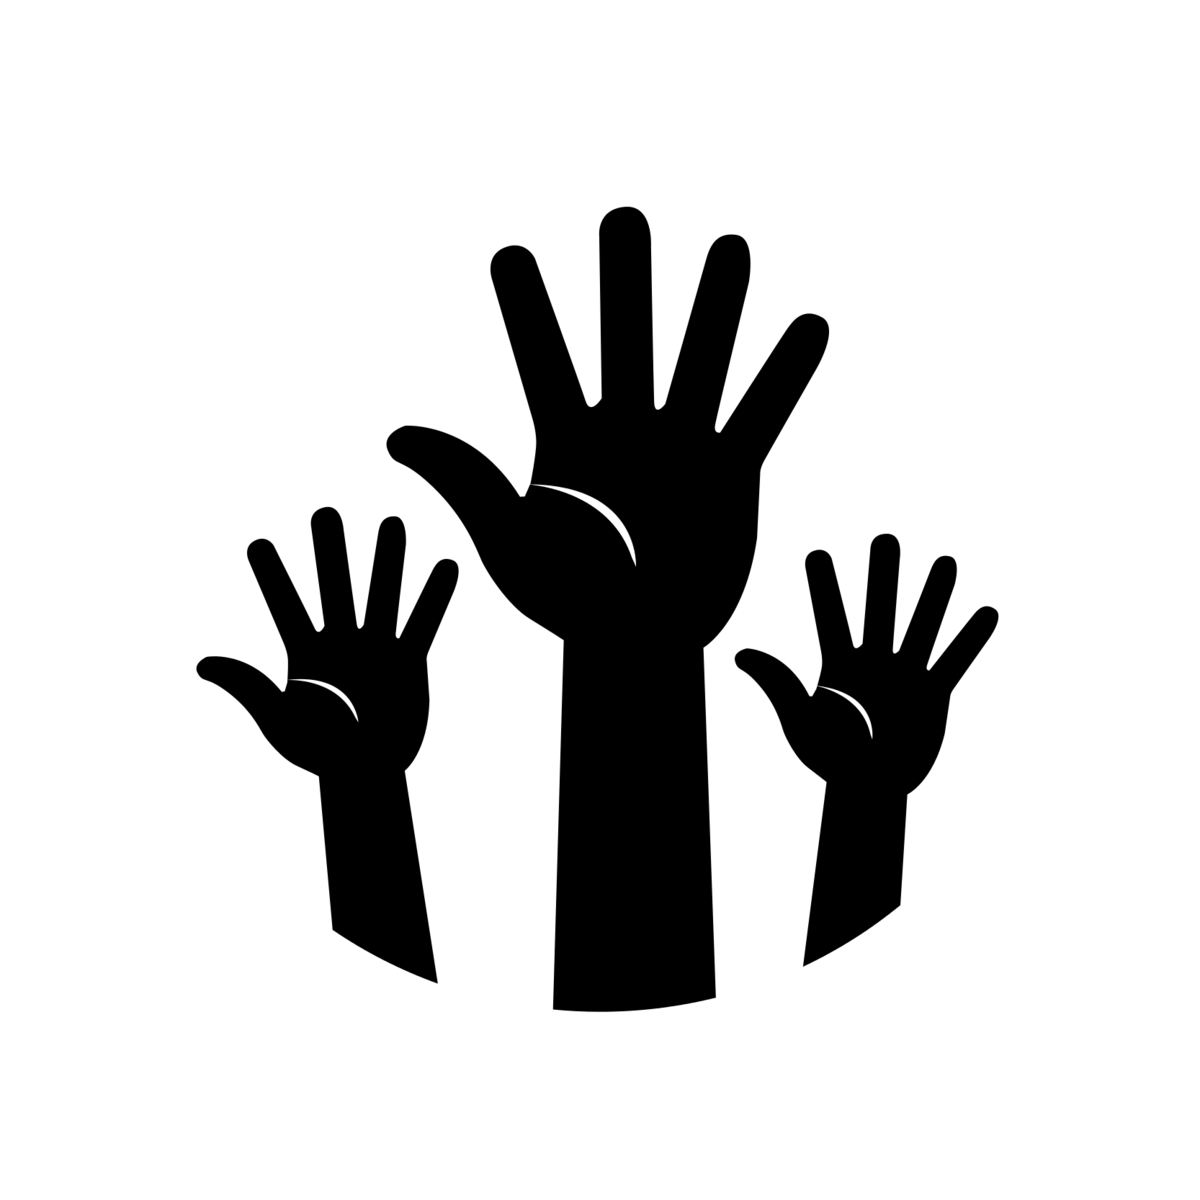
\includegraphics[height=1.5em]{images/hands}}
\newcommand{\transpose}[0]{{\textrm{\tiny{\sf{T}}}}}
\newcommand{\norm}{{\mathcal{N}}}
\newcommand{\cutoff}[0]{\kappa}
\newcommand{\instD}[0]{\dataset}
\newcommand{\insts}[0]{\mathcal{I}}
\newcommand{\inst}[0]{i}
\newcommand{\instI}[1]{i^{(#1)}}

% Iteration specific instance of variable/function/anything
% Introduced in the BO section, but moved up here to make it available within other macros
\newcommand{\iter}[2][\bocount]{{#2}^{(#1)}}

%--------HPO parameter macros-----------

% Parameter Configuration Space
\newcommand{\pcs}[0]{\pmb{\Lambda}}

% ???
\newcommand{\bx}[0]{\conf}

% Parameter Configuration
\newcommand{\conf}[0]{\pmb{\lambda}}

% Final Configuration
\newcommand{\finconf}[0]{\pmb{\hat{\lambda}}}

% Configuration corresponding to a given iteration -- better use \iter!
\newcommand{\confI}[1]{{\conf}^{(#1)}}

% Default Configuration
\newcommand{\defconf}[0]{{\conf}_{\text{def}}}

% Incumbent Configuration
\newcommand{\incumbent}[1][\bocount]{\iter[#1]{\finconf}}

% Optimal Configuration
\newcommand{\optconf}[0]{{\conf}^*}

% Configuration Space
\newcommand{\confs}[0]{\pcs}

%----------------------------------------

%\newcommand{\vlambda}[0]{\bm{\lambda}}
%\newcommand{\vLambda}[0]{\bm{\Lambda}}
\newcommand{\dataset}[0]{\mathcal{D}}
\newcommand{\datasets}[0]{\mathbf{D}}
\newcommand{\loss}[0]{L}
\newcommand{\risk}{\mathcal{R}}
\newcommand{\riske}{\mathcal{R}_{\text{emp}}}
\newcommand{\cost}[0]{c}
\newcommand{\costI}[1]{c^{(#1)}}

% Gaussian Process
\newcommand{\gp}{\mathcal{G}}
% Family of Objective Functions
\newcommand{\objF}{F}

%---------------BO Macros------------------

% BO loop counter
\newcommand{\bocount}{t}
% BO loop counter max, the counter runs from 1 to this value
\newcommand{\bobudget}{T}
% BO loop observation
\newcommand{\obs}[1][\conf]{\cost({#1})}
% BO loop observation space
\newcommand{\obsspace}{\mathcal{Y}}
% BO loop next observation
\newcommand{\bonextobs}{\obs[\iter{\conf}]}
% Acquisition Function, no args
\newcommand{\acq}{u}
% Standard Normal PDF
\newcommand{\pdf}{\phi}
% Standard Normal CDF
\newcommand{\cdf}{\Phi}
% Mean
\newcommand{\mean}{\mu}
% Standard Deviation
\newcommand{\stddev}{\sigma}
% Variance
\newcommand{\variance}{\sigma^2}
% Noise
\newcommand{\noise}{\nu}
% BO loop next selected sample
\newcommand{\bonextsample}{\confI{\bocount}}

% Single hyperparameter
\newcommand{\hyperparam}{\lambda}

% Single hyperparameter within a hyperparameter configuration
\newcommand{\hyperparami}[1][i]{{\hyperparam}_#1}

% Full definition of final configuration
\newcommand{\finconffull}{\incumbent[\bobudget]}

% Dataset
\newcommand{\datasetHPO}{{\dataset}_{HPO}}

% Dataset definition
\newcommand{\datasetHPOdef}{{\langle \bonextsample,\,\bonextobs \rangle}_{\bocount=1}^{\bobudget}}

% Double Display Fraction, forces large displays for everything in numerator and denominator
\newcommand\ddfrac[2]{\frac{\displaystyle #1}{\displaystyle #2}}

% Conditional Probability "Given That" Relation, source:https://tex.stackexchange.com/a/141685/205886
\newcommand\given[1][]{\:#1\vert\:}

% Expectation as a math operator
\DeclareMathOperator*{\E}{\mathbb{E}}

% Citation 
\newcommand{\source}[1]{
    \begin{flushright}
    	Source: \lit{#1}
    \end{flushright}
}
%-------------------------------------------

%Real numbers set
\newcommand{\realnum}{\mathbb{R}}
%Configuration space - do not use
%\newcommand{\configspace}{\Theta}
%Instances - do not use
%\newcommand{\instances}{\mathcal{I}}
%Expected value
\newcommand{\expectation}{\mathbb{E}}
%Kernel
\newcommand{\kernel}{\kappa}
%Constraint function
\newcommand{\constraintf}{c}
%Normal distribution
\newcommand{\normaldist}{\mathcal{N}}

% \renewcommand{\vec}[1]{\mathbf{#1}}
\newcommand{\hist}[0]{\dataset_{\text{Hist}}}
\newcommand{\param}[0]{p}
\newcommand{\algo}[0]{\mathcal{A}}
\newcommand{\algos}[0]{\mathbf{A}}
%\newcommand{\nn}[0]{N}
\newcommand{\feats}[0]{\mathcal{X}_{\text{meta}}}
\newcommand{\feat}[0]{\x_{\text{meta}}}
%\newcommand{\cluster}[0]{\vec{h}}
%\newcommand{\clusters}[0]{\vec{H}}
\newcommand{\perf}[0]{\mathbb{R}}
%\newcommand{\surro}[0]{\mathcal{S}}
\newcommand{\surro}[0]{\hat{\cost}}
\newcommand{\func}[0]{f}
\newcommand{\epm}[0]{\surro}
\newcommand{\portfolio}[0]{\mathbf{P}}
\newcommand{\schedule}[0]{\mathcal{S}}

% Machine Learning
\newcommand{\mdata}[0]{\dataset_{\text{meta}}}
\newcommand{\datasettrain}[0]{\dataset_{\text{train}}}
\newcommand{\datasetval}[0]{\dataset_{\text{val}}}
\newcommand{\datasettest}[0]{\dataset_{\text{test}}}
\newcommand{\x}[0]{\mathbf{x}}
\newcommand{\y}[0]{y}
\newcommand{\xI}[1]{\mathbf{x}^{(#1)}}
\newcommand{\yI}[1]{y^{(#1)}}
\newcommand{\fx}{f(\mathbf{x})}  % f(x), continuous prediction function
\newcommand{\Hspace}{\mathcal{H}} % hypothesis space where f is from
\newcommand{\fh}{\hat{f}}       % f hat, estimated prediction function

% Deep Learning
\newcommand{\weights}[0]{\theta}
\newcommand{\metaweights}[0]{\phi}


% reinforcement learning
\newcommand{\policies}[0]{\mathbf{\Pi}}
\newcommand{\policy}[0]{\pi}
\newcommand{\actionRL}[0]{a}
\newcommand{\stateRL}[0]{s}
\newcommand{\statesRL}[0]{\mathcal{S}}
\newcommand{\rewardRL}[0]{r}
\newcommand{\rewardfuncRL}[0]{\mathcal{R}}

\RestyleAlgo{algoruled}
\DontPrintSemicolon
\LinesNumbered
\SetAlgoVlined
\SetFuncSty{textsc}

\SetKwInOut{Input}{Input}
\SetKwInOut{Output}{Output}
\SetKw{Return}{return}

%\newcommand{\changed}[1]{{\color{red}#1}}

%\newcommand{\citeN}[1]{\citeauthor{#1}~(\citeyear{#1})}

\renewcommand{\vec}[1]{\mathbf{#1}}
\DeclareMathOperator*{\argmin}{arg\,min}
\DeclareMathOperator*{\argmax}{arg\,max}

%\newcommand{\aqme}{\textit{AQME}}
%\newcommand{\aslib}{\textit{ASlib}}
%\newcommand{\llama}{\textit{LLAMA}}
%\newcommand{\satzilla}{\textit{SATzilla}}
%\newcommand{\satzillaY}[1]{\textit{SATzilla'{#1}}}
%\newcommand{\snnap}{\textit{SNNAP}}
%\newcommand{\claspfolioTwo}{\textit{claspfolio~2}}
%\newcommand{\flexfolio}{\textit{FlexFolio}}
%\newcommand{\claspfolioOne}{\textit{claspfolio~1}}
%\newcommand{\isac}{\textit{ISAC}}
%\newcommand{\eisac}{\textit{EISAC}}
%\newcommand{\sss}{\textit{3S}}
%\newcommand{\sunny}{\textit{Sunny}}
%\newcommand{\ssspar}{\textit{3Spar}}
%\newcommand{\cshc}{\textit{CSHC}}
%\newcommand{\cshcpar}{\textit{CSHCpar}}
%\newcommand{\measp}{\textit{ME-ASP}}
%\newcommand{\aspeed}{\textit{aspeed}}
%\newcommand{\autofolio}{\textit{AutoFolio}}
%\newcommand{\cedalion}{\textit{Cedalion}}
\newcommand{\fanova}{\textit{fANOVA}}
\newcommand{\sbs}{\textit{SB}}
\newcommand{\oracle}{\textit{VBS}}

% like approaches
\newcommand{\claspfoliolike}[1]{\texttt{claspfolio-#1-like}}
\newcommand{\satzillalike}[1]{\texttt{SATzilla'#1-like}}
\newcommand{\isaclike}{\texttt{ISAC-like}}
\newcommand{\ssslike}{\texttt{3S-like}}
\newcommand{\measplike}{\texttt{ME-ASP-like}}

\newcommand{\irace}{\textit{I/F-race}}
\newcommand{\gga}{\textit{GGA}}
\newcommand{\smac}{\textit{SMAC}}
\newcommand{\paramils}{\textit{ParamILS}}
\newcommand{\spearmint}{\textit{Spearmint}}
\newcommand{\tpe}{\textit{TPE}}


\usepackage{pifont}
\newcommand{\itarrow}{\mbox{\Pisymbol{pzd}{229}}}
\newcommand{\ithook}{\mbox{\Pisymbol{pzd}{52}}}
\newcommand{\itcross}{\mbox{\Pisymbol{pzd}{56}}}
\newcommand{\ithand}{\mbox{\raisebox{-1pt}{\Pisymbol{pzd}{43}}}}

%\DeclareMathOperator*{\argmax}{arg\,max}

\newcommand{\ie}{{\it{}i.e.\/}}
\newcommand{\eg}{{\it{}e.g.\/}}
\newcommand{\cf}{{\it{}cf.\/}}
\newcommand{\wrt}{\mbox{w.r.t.}}
\newcommand{\vs}{{\it{}vs\/}}
\newcommand{\vsp}{{\it{}vs\/}}
\newcommand{\etc}{{\copyedit{etc.}}}
\newcommand{\etal}{{\it{}et al.\/}}

\newcommand{\pscProc}{{\bf procedure}}
\newcommand{\pscBegin}{{\bf begin}}
\newcommand{\pscEnd}{{\bf end}}
\newcommand{\pscEndIf}{{\bf endif}}
\newcommand{\pscFor}{{\bf for}}
\newcommand{\pscEach}{{\bf each}}
\newcommand{\pscThen}{{\bf then}}
\newcommand{\pscElse}{{\bf else}}
\newcommand{\pscWhile}{{\bf while}}
\newcommand{\pscIf}{{\bf if}}
\newcommand{\pscRepeat}{{\bf repeat}}
\newcommand{\pscUntil}{{\bf until}}
\newcommand{\pscWithProb}{{\bf with probability}}
\newcommand{\pscOtherwise}{{\bf otherwise}}
\newcommand{\pscDo}{{\bf do}}
\newcommand{\pscTo}{{\bf to}}
\newcommand{\pscOr}{{\bf or}}
\newcommand{\pscAnd}{{\bf and}}
\newcommand{\pscNot}{{\bf not}}
\newcommand{\pscFalse}{{\bf false}}
\newcommand{\pscEachElOf}{{\bf each element of}}
\newcommand{\pscReturn}{{\bf return}}

%\newcommand{\param}[1]{{\sl{}#1}}
\newcommand{\var}[1]{{\it{}#1}}
\newcommand{\cond}[1]{{\sf{}#1}}
%\newcommand{\state}[1]{{\sf{}#1}}
%\newcommand{\func}[1]{{\sl{}#1}}
\newcommand{\set}[1]{{\Bbb #1}}
%\newcommand{\inst}[1]{{\tt{}#1}}
\newcommand{\myurl}[1]{{\small\sf #1}}

\newcommand{\Nats}{{\Bbb N}}
\newcommand{\Reals}{{\Bbb R}}
\newcommand{\extset}[2]{\{#1 \; | \; #2\}}

\newcommand{\vbar}{$\,\;|$\hspace*{-1em}\raisebox{-0.3mm}{$\,\;\;|$}}
\newcommand{\vendbar}{\raisebox{+0.4mm}{$\,\;|$}}
\newcommand{\vend}{$\,\:\lfloor$}


\newcommand{\goleft}[2][.7]{\parbox[t]{#1\linewidth}{\strut\raggedright #2\strut}}
\newcommand{\rightimage}[2][.3]{\mbox{}\hfill\raisebox{1em-\height}[0pt][0pt]{\includegraphics[width=#1\linewidth]{#2}}\vspace*{-\baselineskip}}





\newcommand{\inducer}{\mathcal{I}}

\newenvironment{blocki}[1]   % itemize block
{
 \begin{block}{#1}\begin{itemize}
}
{
\end{itemize}\end{block}
}

\title[AutoML: Hyperparameter Optimization]{AutoML: Hyperparameter Optimization}
\subtitle{Overview for this Week}
%TODO: change authors!
\author[Marius Lindauer]{Bernd Bischl \and Frank Hutter \and Lars Kotthoff \and \underline{Marius Lindauer}}
\institute{}
\date{}



% \AtBeginSection[] % Do nothing for \section*
% {
% \begin{frame}{Outline}
% \bigskip
% \vfill
% \tableofcontents[currentsection]
% \end{frame}
% }

\begin{document}

\maketitle


%----------------------------------------------------------------------
%----------------------------------------------------------------------

\begin{frame}[containsverbatim,allowframebreaks]{Motivating Example}

\begin{itemize}
\item Given a dataset, we want to train a classification tree.
\item We feel that a maximum tree depth of $4$ has worked out well for us previously, so we decide to set this hyperparameter to $4$.
\item The learner ("inducer") $\inducer$ takes the input data, internally performs \textbf{empirical risk minimization}, and returns a fitted tree model $\fh(\mathbf{x}) = f(\x, \hat{\theta})$ of at most depth $\lambda = 4$ that minimizes the empirical risk.
\end{itemize}

% FIGURE SOURCE: https://docs.google.com/presentation/d/14xwcs5zncTjFL4hIHAprjZMmyGIPqk5vs8DS32vEAvQ/edit?usp=sharing
\begin{center}
\begin{figure}
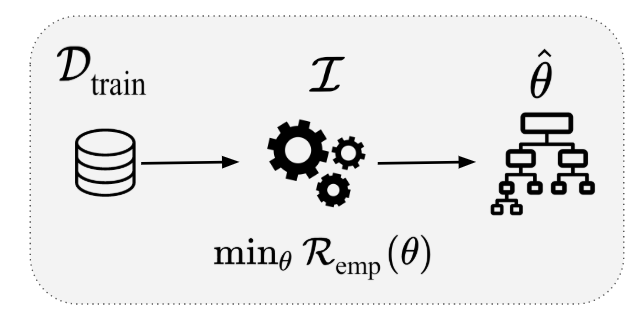
\includegraphics[width=0.6\textwidth]{images/riskmin_bilevel1.png}
\end{figure}
\end{center}

\framebreak

\begin{itemize}
\item We are \textbf{actually} interested in the \textbf{generalization performance} $GE\left(\fh\right)$ of the estimated model on new, previously unseen data.
\item We estimate the generalization performance by evaluating the model $\fh$ on a test set $\datasettest$: $$
\widehat{GE}_{\datasettest}\left(\fh\right) = \frac{1}{|\datasettest|} \sum\limits_{(\x, y) \in \datasettest} L\left(y, \fh(\mathbf{x}) \right)
$$
\end{itemize}
\vspace*{-0.6cm}
% FIGURE SOURCE: https://docs.google.com/presentation/d/14xwcs5zncTjFL4hIHAprjZMmyGIPqk5vs8DS32vEAvQ/edit?usp=sharing
\begin{center}
\begin{figure}
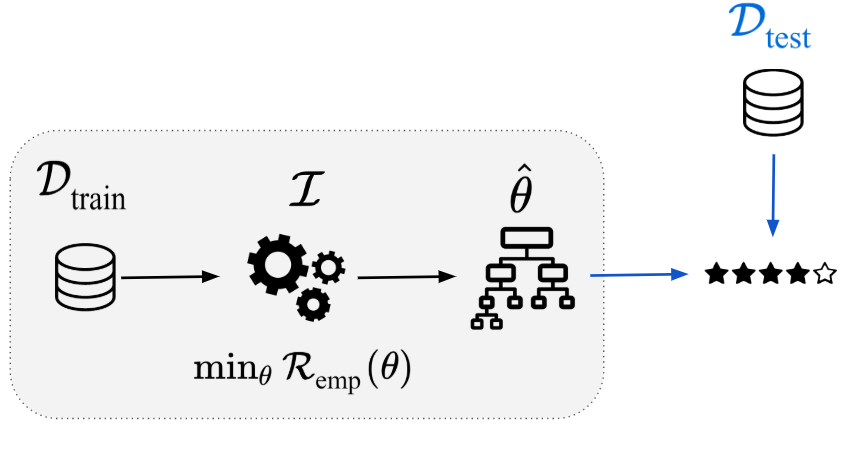
\includegraphics[width=0.75\textwidth]{images/riskmin_bilevel2.png}
\end{figure}
\end{center}

\framebreak

\begin{itemize}
\item But many ML algorithms are sensitive w.r.t. a good setting of their hyperparameters,
and generalization performance might be bad, if we have chosen a suboptimal configuration:
\begin{itemize}
\item The data may be too complex to be modeled by a tree of depth $4$
\item The data may be much simpler than we thought, and a tree of depth $4$ overfits
\end{itemize}
\item[$\implies$] algorithmically try out different values for the tree depth. For each maximal depth $\lambda$, we have to train the model \textbf{to completion} and evaluate its performance on the test set.
\item We choose the tree depth $\conf$ that is \textbf{optimal} w.r.t. the generalization error of the model.
\end{itemize}

% $\to$ Finding the hyperparameter $\lambda$ that is optimal w.r.t. the generalization performance constitutes an optimization problem.

\end{frame}

% \begin{frame}[containsverbatim,allowframebreaks]{The role of hyperparameters}

% \begin{itemize}
% \item Hyperparameters often control the complexity of a model, i.e., how flexible the model is.
% \item But they can in principle influence any structural property of a model or computational part of the training process.
% \item If a model is not flexible enough, it cannot approximate the relationship between the features and the output well and will underfit.
% \item If a model is too flexible so that it simply \enquote{memorizes} the training data, we will face the dreaded problem of overfitting.
% \item[$\implies$] Hence, controlling the model's capacity, i.e., finding suitable hyperparameters,
% can prevent overfitting the model on the training set.
% \end{itemize}

% \end{frame}

\begin{frame}[containsverbatim,allowframebreaks]{Model Parameters vs. Hyperparameters}

It is critical to understand the difference between model parameters and hyperparameters.

\vspace{0.5cm}

\textbf{Model parameters} are optimized during training, typically via loss minimization. They are an \textbf{output} of the training. Examples:
\begin{itemize}
\item The splits and terminal node constants of a tree learner
\item Coefficients $\theta$ of a linear model $\fx = \theta^\top\x$
\end{itemize}

\framebreak

In contrast, \textbf{hyperparameters} (HPs) are not decided during training. They must be specified before the training, they are an \textbf{input} of the training.
Hyperparameters often control the complexity of a model, i.e., how flexible the model is.
But they can in principle influence any structural property of a model or computational part of the training process.

\vspace{0.5cm}

Examples:

\begin{itemize}
\item The maximum depth of a tree
\item $k$ and which distance measure to use for $k$-NN
\item the number and maximal order of interactions to be included in a linear regression model
\end{itemize}

\end{frame}


\begin{frame}[containsverbatim,allowframebreaks]{Types of hyperparameters}

We summarize all hyperparameters we want to tune over in a vector $\conf \in \Lambda$ of (possibly) mixed type. HPs can have different types:

\begin{itemize}
\item Real-valued parameters, e.g.:
\begin{itemize}
\item Minimal error improvement in a tree to accept a split
\item Bandwidths of the kernel density estimates for Naive Bayes
\end{itemize}
\item Integer parameters, e.g.:
\begin{itemize}
\item Neighborhood size $k$ for $k$-NN
\item $mtry$ in a random forest
\end{itemize}
\item Categorical parameters, e.g.:
\begin{itemize}
\item Which split criterion for classification trees?
\item Which distance measure for $k$-NN?
\end{itemize}
\end{itemize}

Hyperparameters are often \textbf{hierarchically dependent} on each other, e.g., \emph{if} we use
a kernel-density estimate for Naive Bayes, what is its width?
% with polynomials of the features up to a certain maximal degree $d$, then
% we must specify whether to also include polynomial interaction terms like e.g. $x_j^{d-d'}x_m^{d'}$ or not
% and up to which degree $d' \leq d$.
\end{frame}

\begin{frame}{Tuning}

\vskip 3em
Recall: \textbf{Hyperparameters} $\conf$ are parameters that are \emph{inputs} to the
training problem, in which a learner $\inducer$ minimizes the empirical risk on a training data set in order
to find optimal \textbf{model parameters} $\theta$ which define the fitted model $\fh$.
\vskip 2em

\textbf{(Hyperparameter) Tuning} is the process of finding good model hyperparameters $\conf$.

% \begin{frame}[containsverbatim,allowframebreaks]{{Hyperparameter Tuning}
% \begin{itemize}
% \item Optimize hyperparameters for learner w.r.t. prediction error
% Tuner proposes configuration, eval by resampling, tuner receives performance, iterate
% \end{itemize}
% \begin{columns}[c, onlytextwidth]
% \column{0.45\textwidth}
% FIGURE SOURCE: No source
% \includegraphics[trim={0cm 0cm 0cm 0cm}, clip, width=1.2\textwidth]{images/chain.jpg}
% \column{0.45\textwidth}
% FIGURE SOURCE: https://drive.google.com/open?id=1wY3aUZxIMZPje3vR0t2yWiDMx_osXRCi
% \includegraphics[trim={1cm 0cm 1cm 0cm}, clip, width=1.2\textwidth]{images/tuning_process.jpg}
% \end{columns}

% \end{frame}

\end{frame}


\begin{frame}[containsverbatim,allowframebreaks]{Tuning: A bi-level optimization problem}

\vspace{0.2cm}

We face a \textbf{bi-level} optimization problem: The well-known risk minimization problem to find $\hat f$ is \textbf{nested} within the outer hyperparameter optimization (also called second-level problem):

\begin{center}
\begin{figure}
% FIGURE SOURCE: https://docs.google.com/presentation/d/14xwcs5zncTjFL4hIHAprjZMmyGIPqk5vs8DS32vEAvQ/edit?usp=sharing
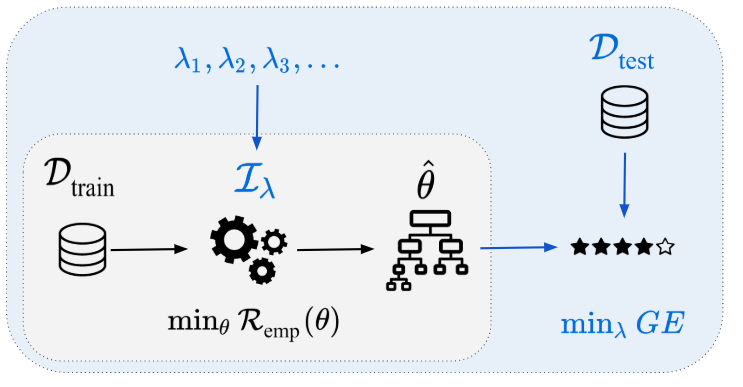
\includegraphics[width=0.8\textwidth]{images/riskmin_bilevel3.png}
\end{figure}
\end{center}

\framebreak

\begin{itemize}
\item For a learning algorithm $\inducer$ (also inducer) with $d$ hyperparameters, the hyperparameter \textbf{configuration space} is:
$$\Lambda=\Lambda_{1} \times \Lambda_{2} \times \ldots \Lambda_{d}$$
where $\Lambda_{i}$ is the domain of the $i$-th hyperparameter.
\item The domains can be continuous, discrete or categorical.
\item For practical reasons, the domain of a continuous or integer-valued hyperparameter is typically bounded.
\item A vector in this configuration space is denoted as $\conf \in \Lambda$.
\item A learning algorithm $\inducer$ takes a (training) dataset $\dataset$ and a hyperparameter configuration $\conf \in \Lambda$ and returns a trained model (through risk minimization)

\vspace*{-0.2cm}
\begin{eqnarray*}
\inducer: \left(\mathcal{X} \times \mathcal{Y}\right)^n \times \Lambda &\to& \mathcal{H} \\
(\dataset, \Lambda) &\mapsto& \inducer(\dataset, \Lambda) = \hat f_{\dataset, \Lambda}
\end{eqnarray*}
% \item Additionally, some hyperparameters may only need to be specified if another hyperparameter (or combination of hyperparameters) takes on a certain value.
\end{itemize}

% \lz

% Note that

% In contrast to the first-level (empirical) risk minimization problem, hyperparameter optimization is also referred to as \textbf{second-level} optimization. The first-level problem can be seen as a subroutine called by the second-level problem: Each evaluation of $\Lambda$ requires to solve the first-level optimization problem.


% \framebreak

% \begin{itemize}
% \item search for the \textbf{inducer} hyperparameter $\Lambda$
% \item that minimizes the \textbf{generalization error}
% $$
% \min_{\Lambda} \E_{\D_n \sim \Pxy, (\xv, y) \sim \Pxy} \left(V\left(y, \hat f_{\D, \Lambda}(\xv)\right)\right).
% $$
% \end{itemize}

% We compare: In empirical risk minimization, we

% \begin{itemize}
% \item search for the \textbf{model} parameter $\thetab$
% \item that minimizes the \textbf{empirical risk}
% $$
% \min_{\thetab} \sum_{(\xi, \yi) \in \datasettrain} L\left(\yi, \fxi\right).
% $$
% \end{itemize}

% In hyperparameter optimization, we

% \begin{itemize}
% \item search for the \textbf{inducer} hyperparameter $\Lambda$
% \item that minimizes the \textbf{test error}
% $$
% \min_{\Lambda \in \Lambda} \sum_{(\xi, \yi) \in \datasettest} V\left(\inducer(\datasettrain, \Lambda)(\xi), \yi\right).
% $$
% \end{itemize}

% \framebreak

% \framebreak

% The hyperparameter optimization problem is difficult in many ways:
\end{frame}


\begin{frame}[containsverbatim,allowframebreaks]{Tuning: A bi-level optimization problem}
We formally state the nested hyperparameter tuning problem as:

$$
\min_{\conf \in \Lambda} \widehat{GE}_{\datasettest}\left(\inducer(\datasettrain, \Lambda)\right)
$$

\begin{itemize}
\item The learner $\inducer(\datasettrain, \conf)$ takes a training dataset as well as hyperparameter settings $\Lambda$ (e.g. the maximal depth of a classification tree) as an input.
\item $\inducer(\datasettrain, \conf)$ performs empirical risk minimization on the training data and returns the optimal model $\hat f$ for the given hyperparameters.
\item Note that for the estimation of the generalization error, more sophisticated resampling strategies like cross-validation can be used.
\end{itemize}

\framebreak

The components of a tuning problem are:

\begin{itemize}
\item The dataset
\item The learner (possibly: several competing learners?) that is tuned %(e.g. a decision tree classifier)
\item The learner's hyperparameters and their respective regions-of-interest over which we optimize % (e.g. $\texttt{tree depth} \in \{1, 2, ..., 20\}$)
\item The performance measure, as determined by the application.\\ Not necessarily identical to the loss function that defines the risk minimization problem for the learner!\\
% We could even be interested in multiple measures simultaneously, e.g., accuracy and computation time of our model, TPR and PPV, etc.
\item A (resampling) procedure for estimating the predictive performance.
 % The expected performance on unseen data can be estimated by holdout (i.e., a single train-test-split) or more advanced techniques like cross-validation.
% More on this later.
\end{itemize}

% \framebreak

% \begin{center}
% \begin{figure}
% FIGURE SOURCE: https://docs.google.com/presentation/d/1JUtguuVBgidcqD0IdFFIiKH9zqYzM6YRjCqC53V90dA/edit?usp=sharing
% 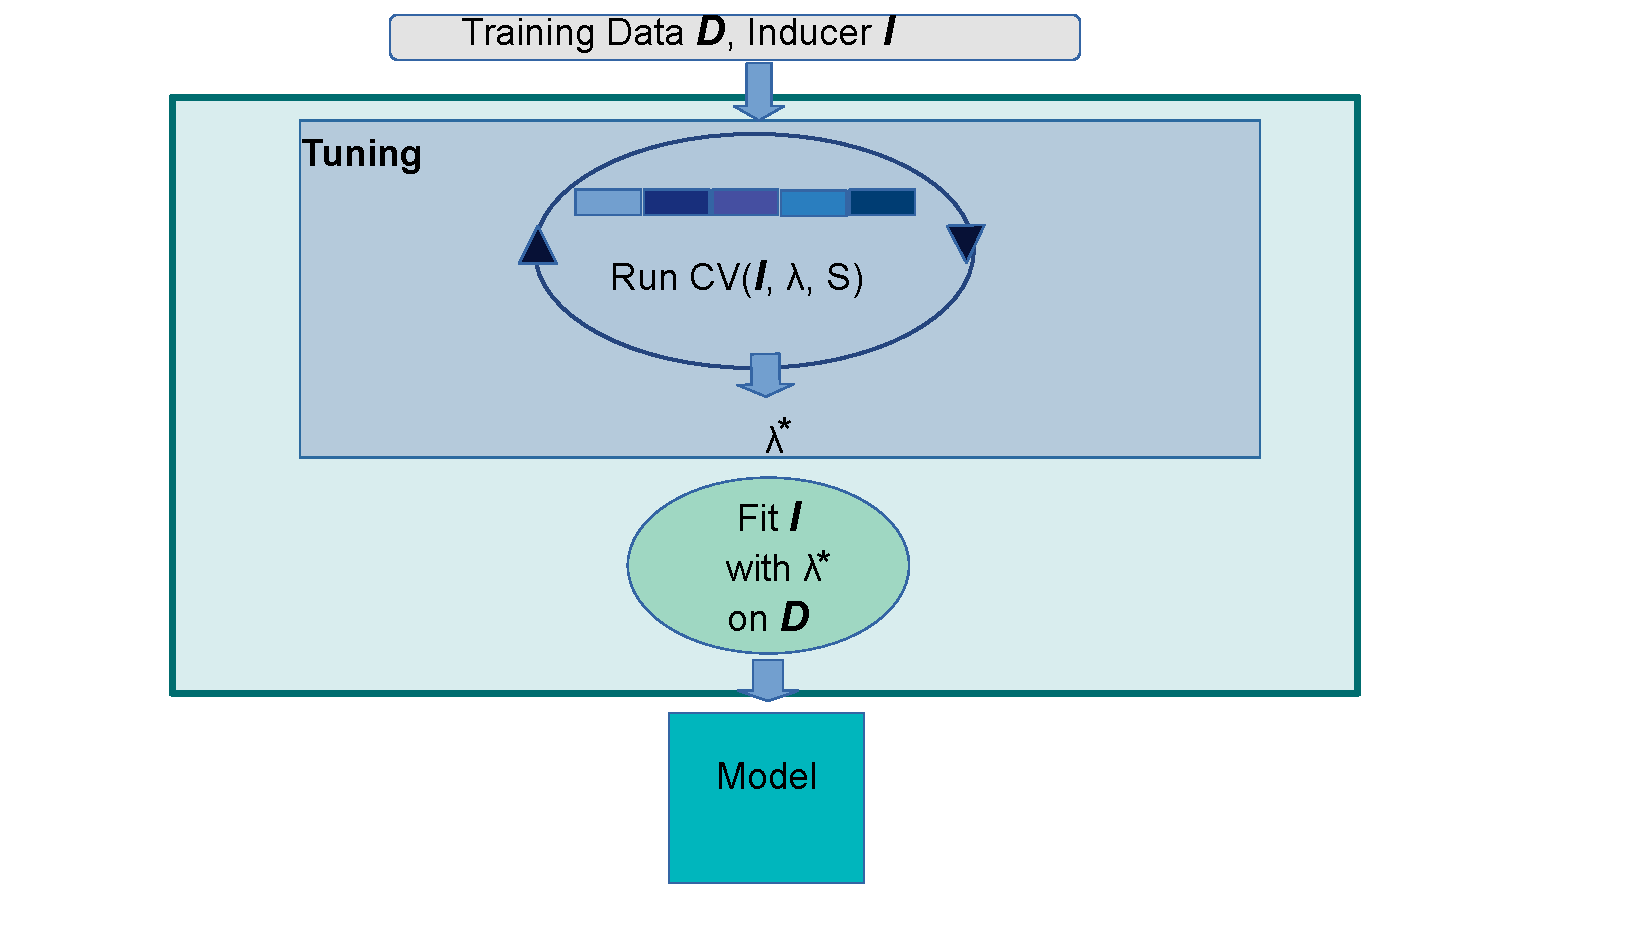
\includegraphics[width=1.2\textwidth]{images/autotune_in_model_fit.pdf}
% \end{figure}
% \end{center}

\end{frame}




% \framebreak

% Possible scenarios for finding default hyperparameters:

% \begin{itemize}
% \item If the learner's performance is fairly insensitive to changes of a hyperparameter, we don't really have to worry as long as we remain within the range of reasonable values.
% \item Constant default: we can benchmark the learner across a broad range of data sets and scenarios and try to find hyperparameter values that work well in many different situations. Quite optimistic?
% \item Dynamic (heuristic) default: We can benchmark the learner across a broad range of data sets and scenarios and try to find an easily computable function that sets the hyperparameter in a data dependent way,
% e.g. using \texttt{mtry}$ = p/3$ for RF.\\
% How to construct or learn that heuristic function, though...?
% \item In some cases, can try to set hyperparameters optimally by extracting more info from the fitted model. E.g. \texttt{ntrees} for a random forest (does OOB error increase or decrease if you remove trees from the ensemble?).
% \end{itemize}
% \end{frame}









\begin{frame}[containsverbatim,allowframebreaks]{Why is tuning so hard?}
\begin{itemize}
\item Tuning is derivative-free (black box problem): It is usually impossible to compute derivatives of the objective (i.e., the resampled performance measure) that we optimize with regard to the HPs. All we can do is evaluate the performance for a given hyperparameter configuration.
\item Every evaluation requires one or multiple train and predict steps of the learner. I.e., every evaluation is very \textbf{expensive}.
\item Even worse: the answer we get from that evaluation is \textbf{not exact, but stochastic} in most settings, as we use resampling.
\item Categorical and dependent hyperparameters aggravate our difficulties: the space of hyperparameters we optimize over has a non-metric, complicated structure.
\end{itemize}

\end{frame}


\begin{frame}[containsverbatim,allowframebreaks]{Grid search}

    \begin{columns}
        \begin{column}{0.49\textwidth}
            \begin{itemize}
                \item Simple technique which is still quite popular, tries all
                HP combinations on a multi-dimensional discretized grid
                \item For each hyperparameter a finite set of candidates is predefined
                \item Then, we simply search all possible combinations in arbitrary order
                \end{itemize}
        \end{column}
        \begin{column}{0.49\textwidth}
            \begin{center}
            \begin{figure}
                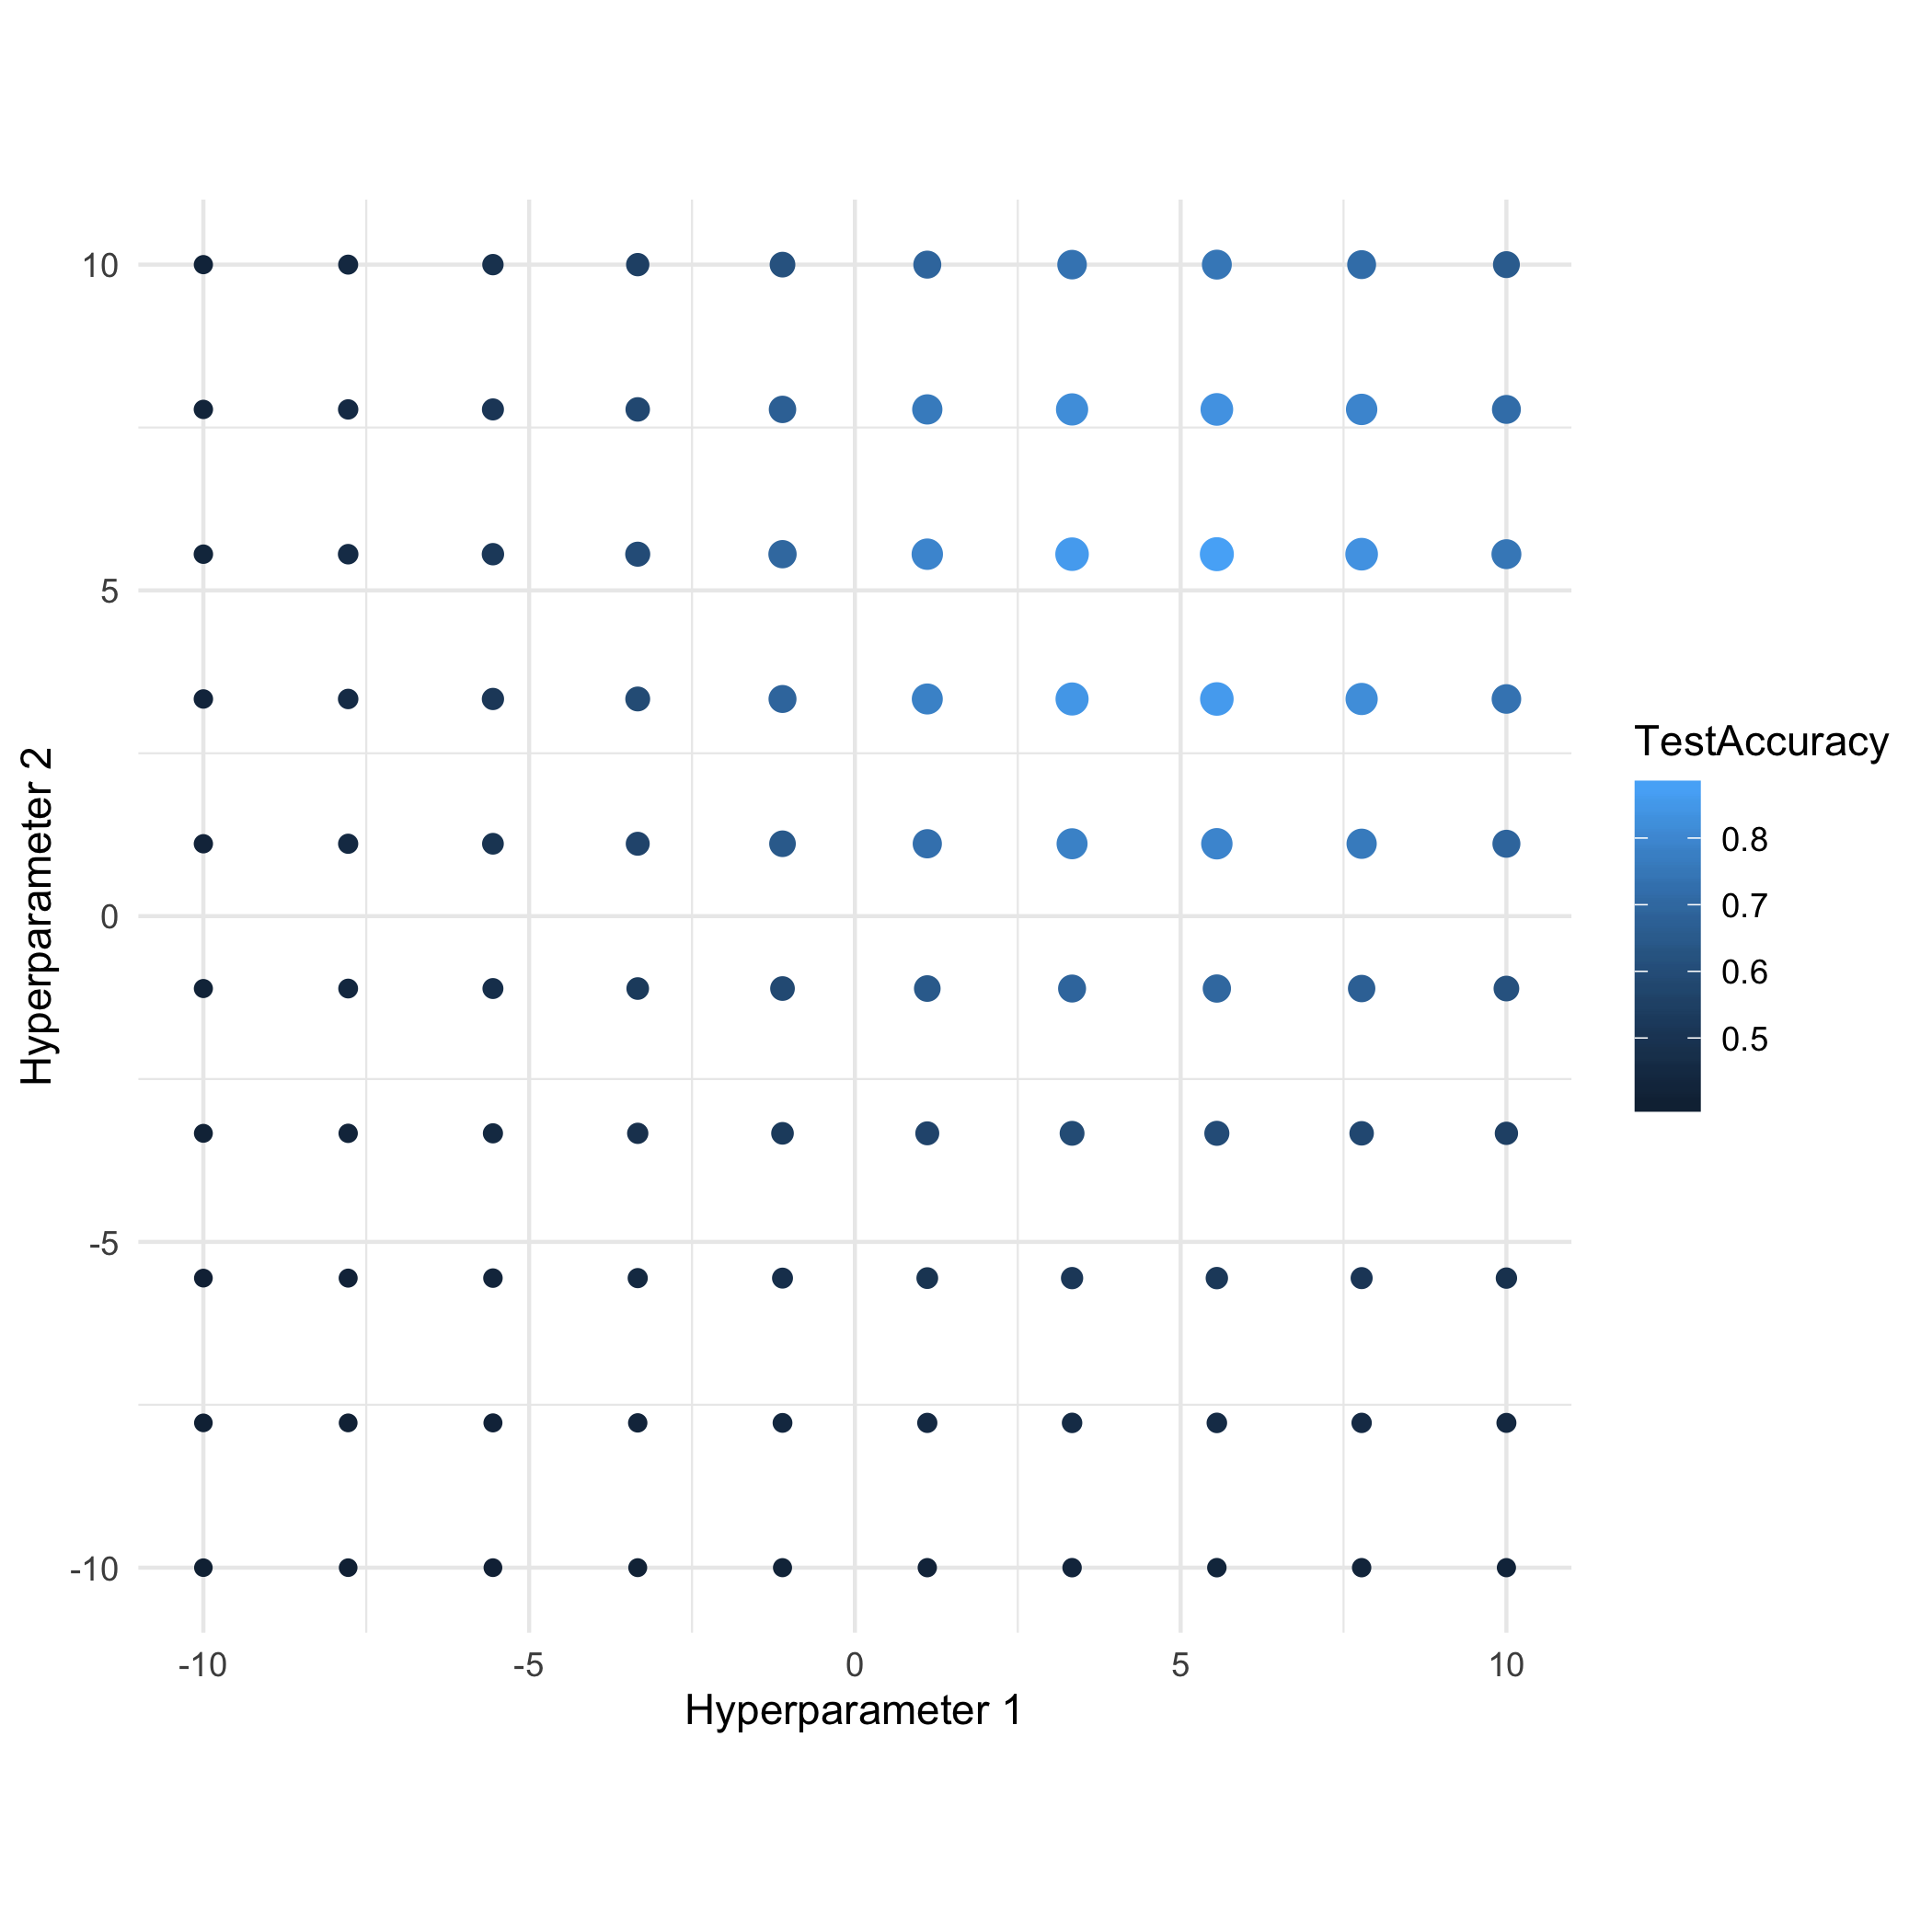
\includegraphics[width=0.8\textwidth]{images/grid.png}
                \caption*{Grid search over 10x10 points}
            \end{figure}
            \end{center}
        \end{column}
    \end{columns}

\framebreak

\begin{blocki}{Advantages}
\item Very easy to implement
\item All parameter types possible
\item Parallelizing computation is trivial
\end{blocki}

\begin{blocki}{Disadvantages}
\item  Scales badly: Combinatorial explosion
\item  Inefficient: Searches large irrelevant areas
\item  Arbitrary: Which values / discretization?
\end{blocki}
\end{frame}


\begin{frame}[containsverbatim,allowframebreaks]{Random search}



    \begin{columns}
        \begin{column}{0.49\textwidth}
            \begin{itemize}
                \item Small variation of grid search
                \item Uniformly sample from the region-of-interest
                \end{itemize}
        \end{column}
        \begin{column}{0.49\textwidth}
            \begin{center}
            \begin{figure}
                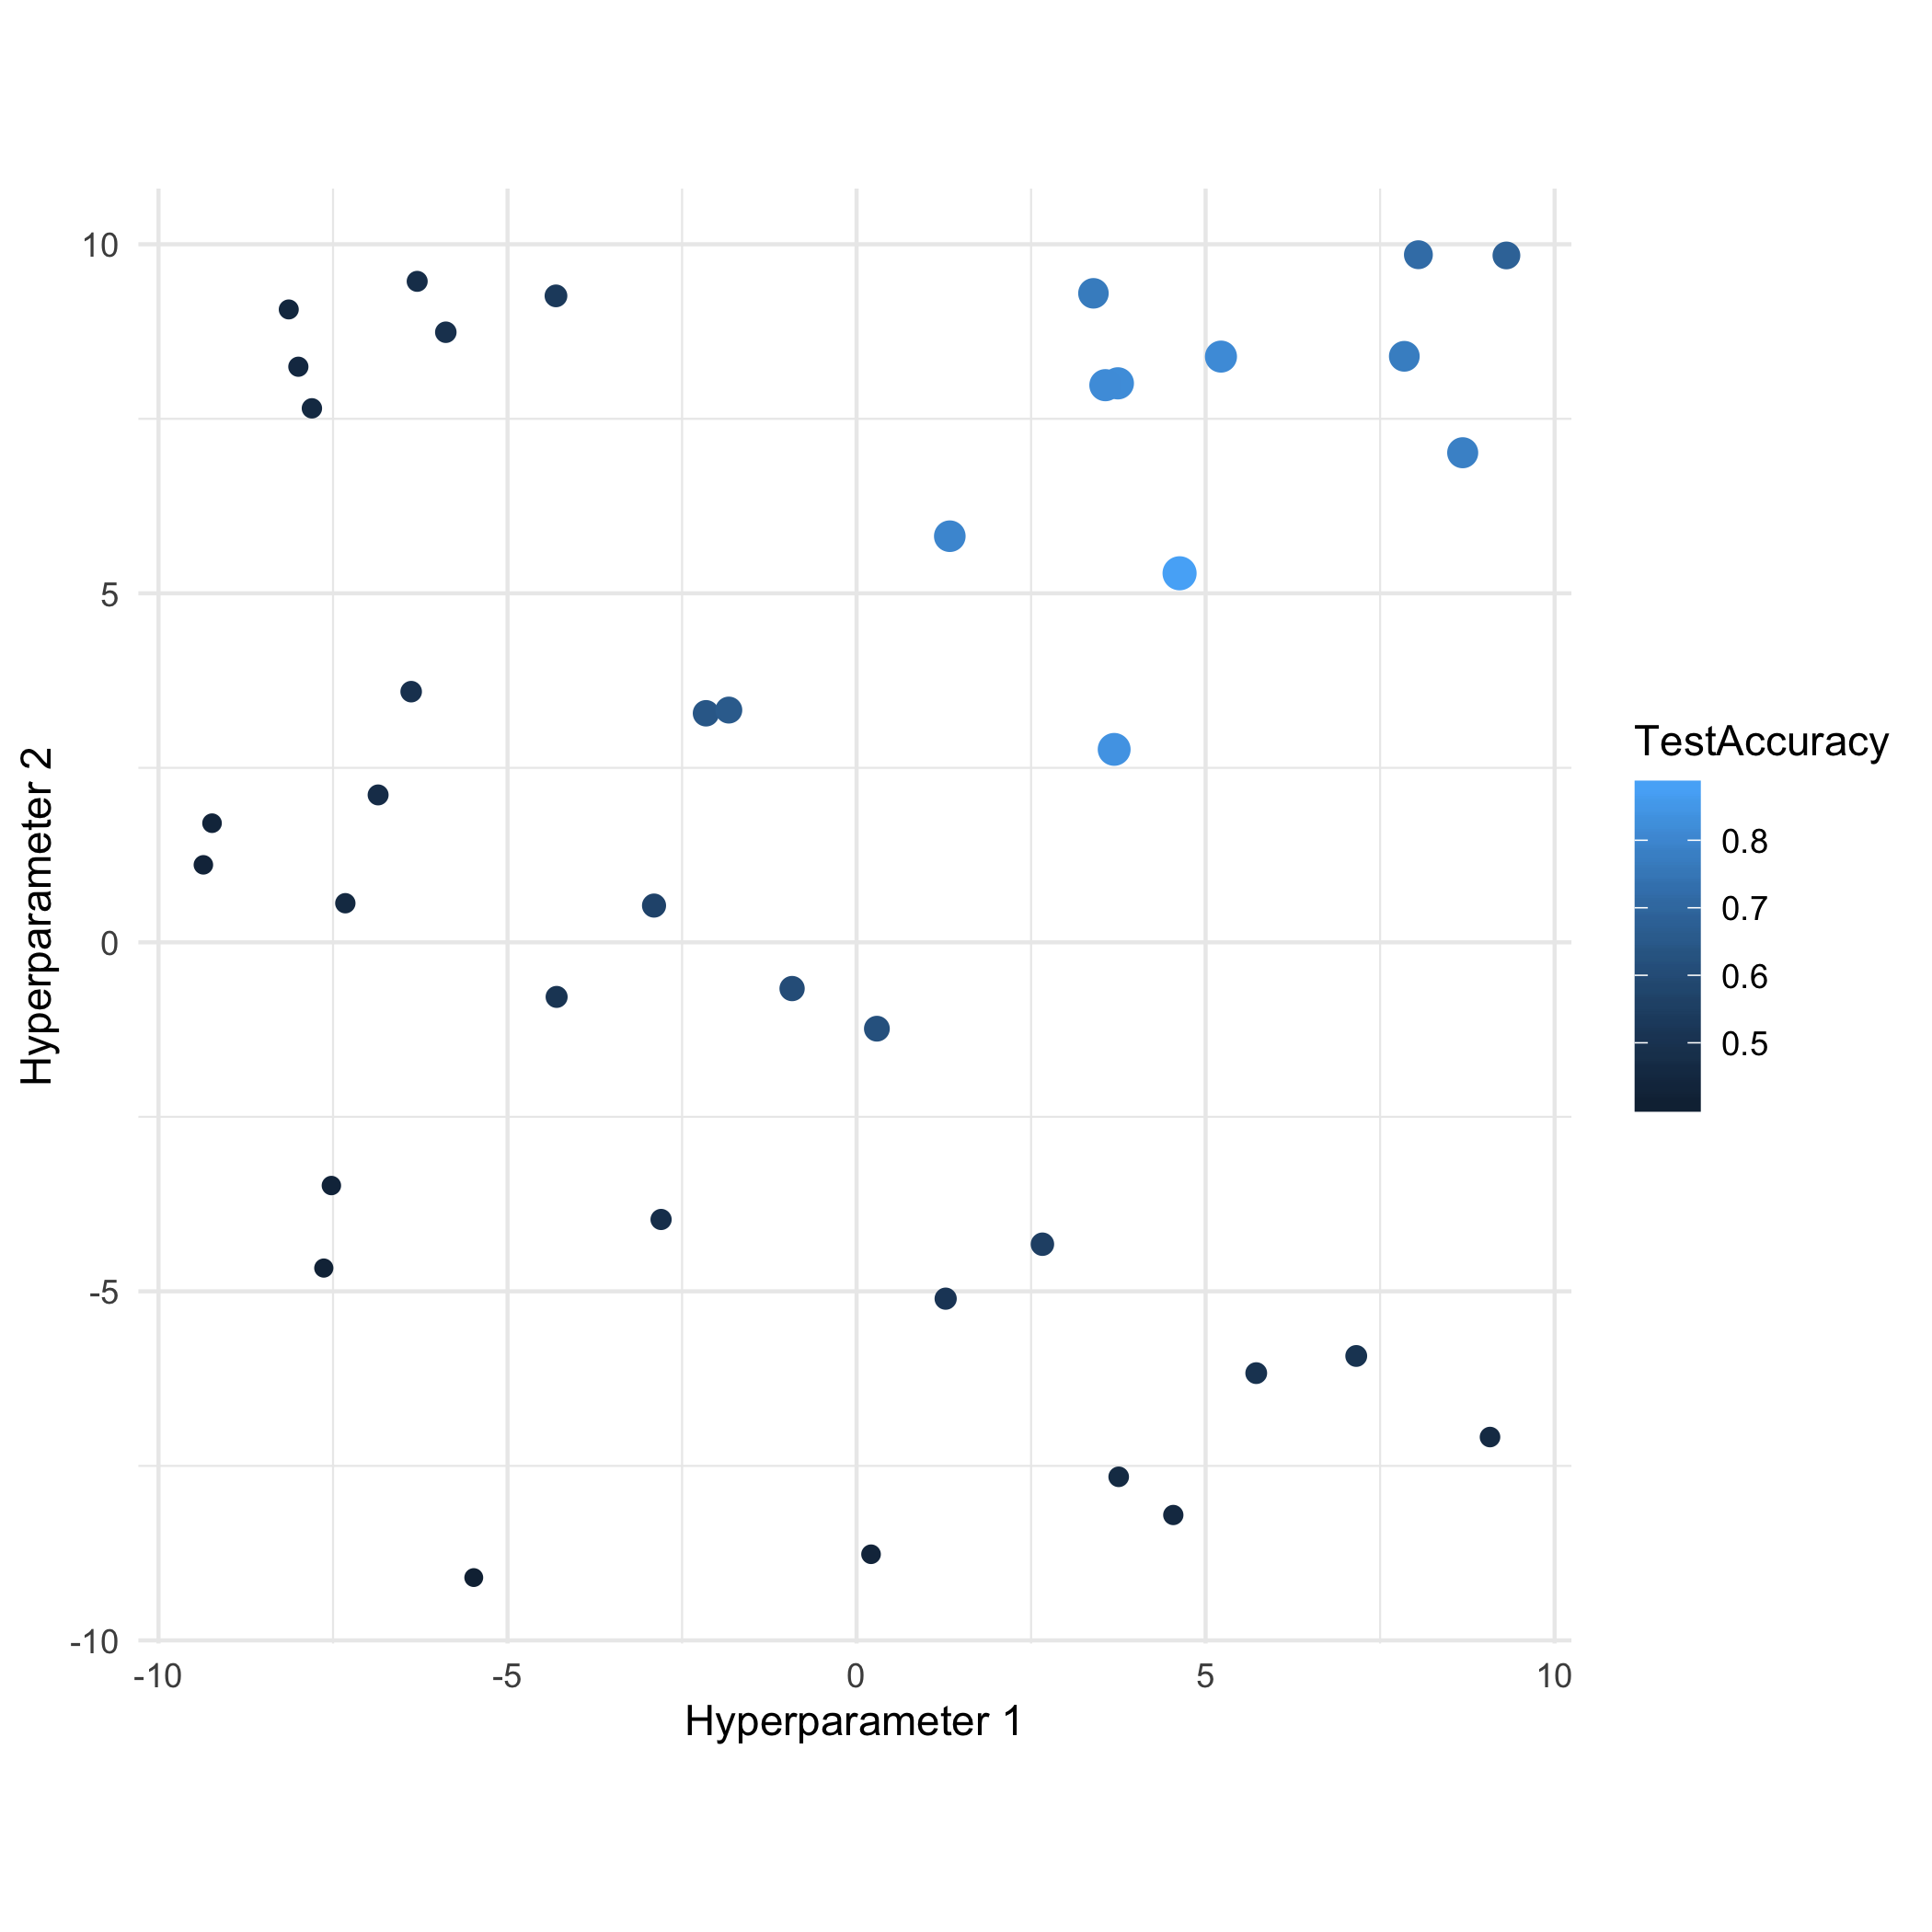
\includegraphics[width=0.8\textwidth]{images/random.png}
                \caption*{Random search over 100 points}
            \end{figure}
            \end{center}
        \end{column}
    \end{columns}

\framebreak

\begin{blocki}{Advantages}
\item Like grid search: Very easy to implement, all parameter types possible, trivial parallelization
\item Anytime algorithm: Can stop the search whenever our budget for computation is exhausted, or continue until we reach our performance goal.
\item No discretization: each individual parameter is tried with a different value every time
\end{blocki}

\begin{blocki}{Disadvantages}
\item Inefficient: many evaluations in areas with low likelihood for improvement
\item Scales badly: high dimensional hyperparameter spaces need \emph{lots} of samples to cover.
\end{blocki}
\end{frame}

\begin{frame}[containsverbatim,allowframebreaks]{Tuning Example}

Tuning random forest with random search and 5CV on the \texttt{sonar} data set for AUC:



\begin{columns}
    \begin{column}{0.49\textwidth}
        \begin{center}
            \begin{tabular}{|l|l|l|l}
            Parameter  &  Type & Min & Max \\
            \hline
            \texttt{num.trees} & integer  & 3 & 500 \\
            \texttt{mtry}  & integer  & 5 & 50  \\
            \texttt{min.node.size} & integer  & 10 & 100\\
            \end{tabular}
            \end{center}
    \end{column}
    \begin{column}{0.49\textwidth}
        \begin{center}
            \begin{figure}
            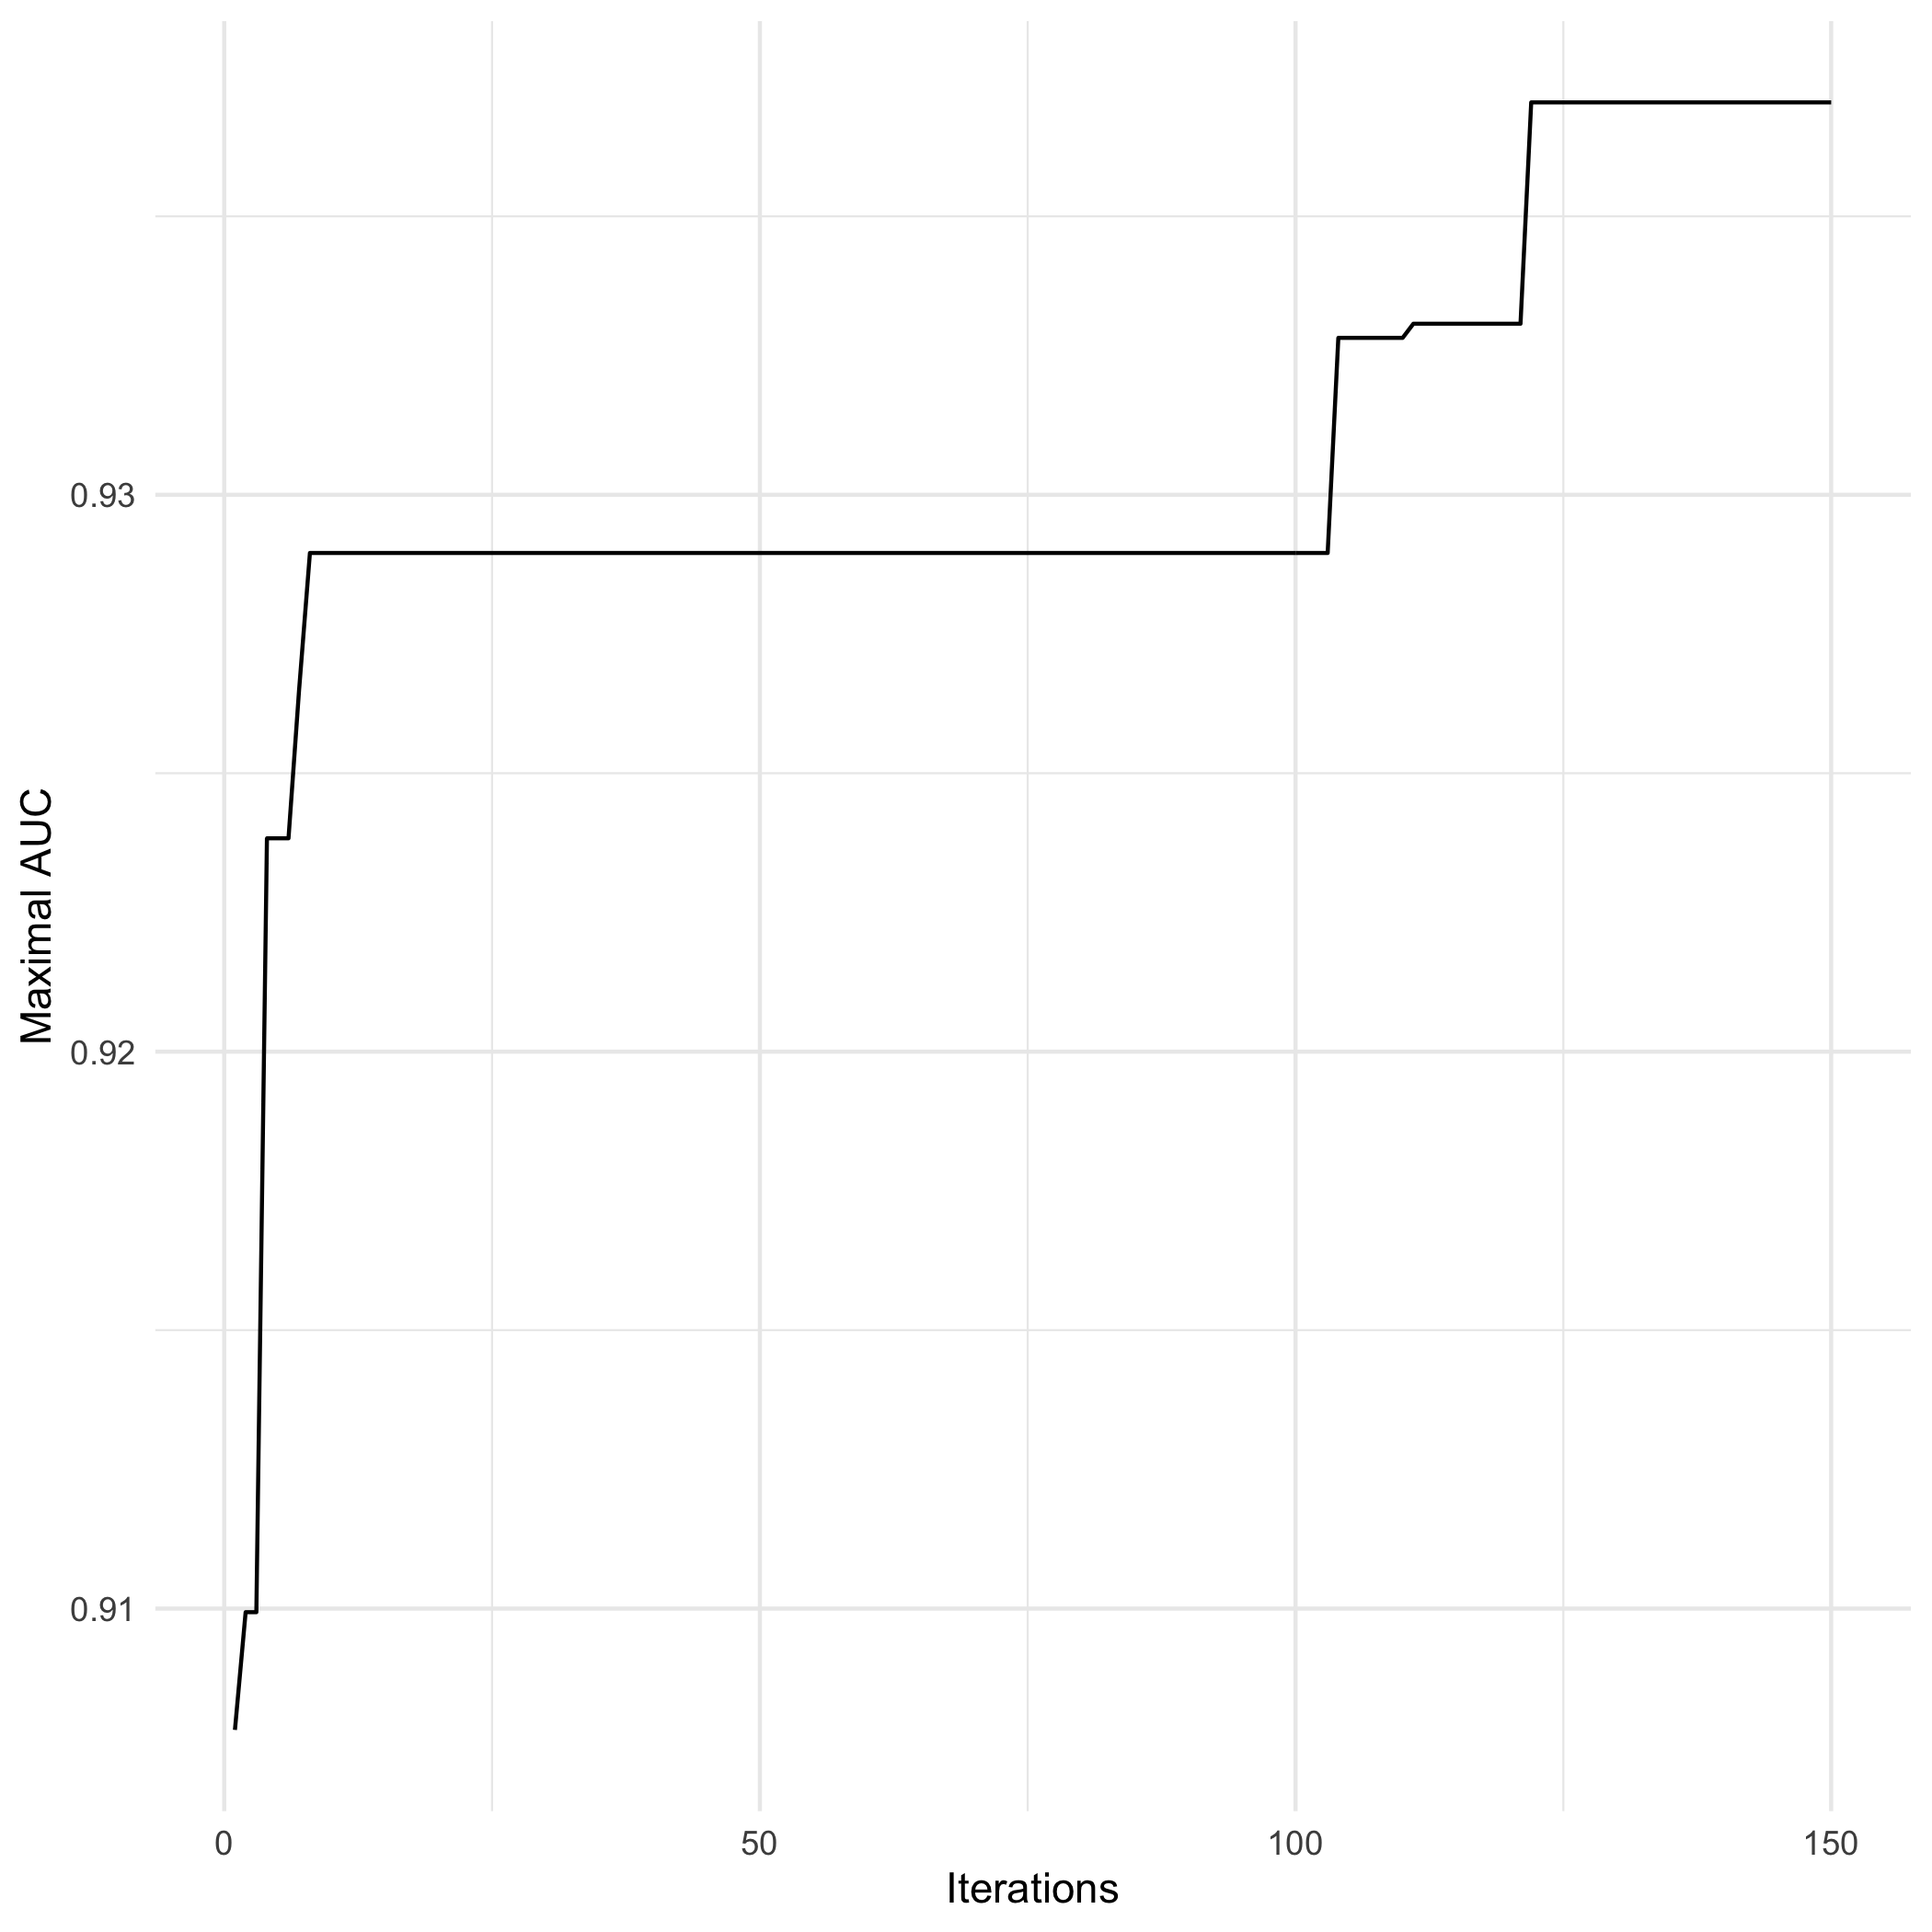
\includegraphics[width=0.8\textwidth]{images/curve.png}
            \end{figure}
            \end{center}
    \end{column}
\end{columns}


\end{frame}



\end{document}
